\documentclass[11pt,a4paper]{article}
\usepackage[utf8]{inputenc}
\usepackage{amsmath}
\usepackage{amsthm}
\usepackage{amsfonts}
\usepackage{amssymb}
%\usepackage{algorithmic}
%\usepackage{algorithm}
\usepackage{hyperref}
%\usepackage[ruled,linesnumbered,procnumbered]{algorithm2e}

\makeatletter
\let\original@algocf@latexcaption\algocf@latexcaption
\long\def\algocf@latexcaption#1[#2]{%
  \@ifundefined{NR@gettitle}{%
    \def\@currentlabelname{#2}%
  }{%
    \NR@gettitle{#2}%
  }%
  \original@algocf@latexcaption{#1}[{#2}]%
}
\makeatother

\usepackage{xcolor}		% for adding colors to the text

\usepackage[footnotesize, center]{caption}	
\usepackage{subcaption}
%\usepackage{subfigure}
\usepackage{booktabs}
\usepackage{multirow}
\usepackage{breakurl}	% fixes the problem of breaking long url into lines inside the bibliography (IMP: must be below the hyperref package)
\hypersetup{
    bookmarks=true,		% show bookmarks bar?
    colorlinks=true,		% false: boxed links; true: colored links
    linkcolor=blue,		% color of internal links
    citecolor=blue,		% color of links to bibliography
    filecolor=blue,		% color of file links
    urlcolor=blue,		% color of external links
    bookmarksopen=true,
    breaklinks=true,
}
%\usepackage{natbib}			% bibliography
%\setlength{\bibsep}{0pt}

\usepackage[title]{appendix}

\usepackage{longtable}

% Page Setup

% Margins
	% MS Word (Default):		[margin=0.98in]
	% MS Word (Narrow):		[margin=0.5in]
\usepackage[margin=2cm]{geometry}
\setlength{\parskip}{\medskipamount}

\usepackage{setspace}
%\onehalfspacing
\setstretch{1.15}

\usepackage{indentfirst}			% indent the first paragraph
\allowdisplaybreaks				% break if equations take too much vertical space

% Section Style
\makeatletter
\def\@seccntformat#1{\csname the#1\endcsname.\quad}		% put a fullstop after section numbers
\makeatother

% Optional packages
\usepackage{xfrac}	% nicer fractional symbols (e.g., \sfrac{1}{2})
\usepackage{fancyhdr}	% adding headers / footers

% MACROS

% mathematical
\newcommand{\mathbold}[1]{\boldsymbol{#1}}		% for adding bold greek letters
\newcommand{\binary}{\{ 0, 1 \} }

\newcommand{\parentheses}[1]{\left( #1 \right) }	% auto-size parentheses
\newcommand{\brackets}[1]{\left[ #1 \right] }		% auto-size brackets
\newcommand{\curly}[1]{\left\{ #1 \right\} }		% auto-size curly brackets

	% Nilay Noyan's commenting macros
	% commentbox (adds black comments in a frame box)
	% comment (adds red comments as a footnote)

\newcounter{commentcounter}
\setcounter{commentcounter}{1}

\setlength{\fboxsep}{5pt}
\setlength{\fboxrule}{0.1pt}

\newcommand{\commentbox}[1]{
% \hfill \newline \noindent
%	\framebox[\textwidth]{
%		\parbox{0.98\textwidth}{
%			\footnotesize{
%				\texttt{\textcolor{black}{(C.\arabic{commentcounter})~#1\hfill}}}}}
%	\addtocounter{commentcounter}{1} 
	}

\long\def\symbolfootnote[#1]#2{\begingroup\def\thefootnote{\fnsymbol{footnote}}\footnote[#1]{#2}\endgroup}

\newcommand{\comment}[2]{{\footnotesize\texttt{\textcolor{red}{(C.\arabic{commentcounter})}}\symbolfootnote[4]{\texttt{\textcolor{red}
        {(C.\arabic{commentcounter}) [#1]: ~#2}}}}\addtocounter{commentcounter}{1}}
%\newcommand{\comment}[2]{}

% theorems
% the subtheorem environment is used to generate theorem numbers 1a, 1b, etc.
% Source: http://tex.stackexchange.com/questions/43346/how-do-i-get-sub-numbering-for-theorems-theorem-1-a-theorem-1-b-theorem-2
\makeatletter
\newenvironment{subtheorem}[1]{%
  \def\subtheoremcounter{#1}%
  \refstepcounter{#1}%
  \protected@edef\theparentnumber{\csname the#1\endcsname}%
  \setcounter{parentnumber}{\value{#1}}%
  \setcounter{#1}{0}%
  \expandafter\def\csname the#1\endcsname{\theparentnumber\alph{#1}}%
  \ignorespaces
}{%
  \setcounter{\subtheoremcounter}{\value{parentnumber}}%
  \ignorespacesafterend
}
\makeatother
\newcounter{parentnumber}
% end of subtheorem environment

\newtheorem{theorem}{\bf Theorem}
\newtheorem{lemma}{\bf Lemma}
\newtheorem{proposition}{\bf Proposition}
\newtheorem{corollary}{\bf Corollary}
\newtheorem{definition}{\sc Definition}
\newtheorem{fact}{\bf Fact}
\newtheorem{claim}{\sc Claim}
\newtheorem{case}{\sc Case}
\newtheorem{observation}{\sc Observation}
\renewcommand{\qedsymbol}{\hfill \tiny$\blacksquare$}		% symbol for proof environment
\renewcommand{\proofname}{\textnormal{\textbf{Proof.}}}	% title in the proof environment

\newtheoremstyle{mytheoremstyle} % name
    {\topsep}                    % Space above
    {\topsep}                    % Space below
    {}                   % Body font
    {}                           % Indent amount
    {\scshape}                   % Theorem head font
    {.}                          % Punctuation after theorem head
    {.5em}                       % Space after theorem head
    {}  % Theorem head spec (can be left empty, meaning ‘normal’)
\theoremstyle{mytheoremstyle}
\newtheorem{example}{Example}

\newtheoremstyle{myassumptionstyle} % name
    {\smallskipamount}                    % Space above
    {0}                    % Space below
    {}                   % Body font
    {}                     	% Indent amount
    {\upshape}              % Theorem head font
    {.}                          	% Punctuation after theorem head
    {.5em}                      % Space after theorem head
    {}  				% Theorem head spec (can be left empty, meaning ‘normal’)
\theoremstyle{myassumptionstyle}
\newtheorem{assumption}{\bf A\ignorespaces}
\newtheorem{remark}{\bf Remark}

\DeclareMathOperator*{\argmin}{arg\,min} 
\DeclareMathOperator*{\argmax}{arg\,max} 


% narrative
\newcommand{\ie}{\textit{i.e.}}		% id est, that is to say
\newcommand{\ex}{\textit{ex.}}		% example
\newcommand{\eg}{\textit{e.g.}}	% exempli gratia, for the sake of example

\newcommand{\st}{\text{subject to:}\qquad}	% subject to
\newcommand{\mathbi}[1]{\boldsymbol{#1}}	% \boldsymbol{ any character } // makes both italic and bold

\newcommand{\cplex}{\texttt{CPLEX}}

\newcommand{\question}[1]{\vspace{\baselineskip}\noindent\pdfbookmark{Question #1}{Question #1}\textbf{\large{Question #1}} \normalsize\medskip\newline}
\newcommand{\qpart}[1]{\indent\textbf{#1)}}	% i.e., a), b), ...

\newcommand{\inlinecomment}[1]{{\color[rgb]{0.13,0.57,0.4} \textbf{#1}}}

% algorithmic
\newcommand{\np}{$\mathcal{NP}$}	% e.g., as in NP-hard

\usepackage{enumitem}	% for aligned descriptions
\usepackage{calc} 		% for aligned descriptions

\setenumerate{
itemsep=0pt,
partopsep=0pt,
parsep=0pt,
topsep=0pt,
labelindent=4pt,
font=\normalfont
}

\setdescription{
itemsep=0pt,
partopsep=0pt,
parsep=0pt,
topsep=0pt,
labelindent=4pt,
font=\normalfont
}

\setitemize{
itemsep=0pt,
partopsep=0pt,
parsep=0pt,
topsep=0pt,
labelindent=4pt,
font=\normalfont
}


\usepackage{natbib}			% bibliography
\setlength{\bibsep}{0pt}

\setlength{\textheight}{23cm} %{23cm}
\setlength{\topmargin}{-2cm}
\setlength{\textwidth}{17.5cm} \setlength{\oddsidemargin}{-0.5cm}
\setlength{\evensidemargin}{-0.5cm}

\setlength{\parindent}{0pt}

\newcommand{\gap}{\vspace{5pt}}
\newcommand{\epc}{\hspace{1pc}}

\newcommand{\onebld}{{\bf 1}}
\newcommand{\wt}{\widetilde}
\newcommand{\wh}{\widehat}

\usepackage{moreverb} % for verbatim ouput
% Count of words
\immediate\write18{texcount -inc -incbib 
-sum writeup.tex > /tmp/wordcount.tex}
\newcommand\wordcount{
\verbatiminput{/tmp/wordcount.tex}}

% Count of characters
\immediate\write18{texcount -char -freq
 writeup.tex > /tmp/charcount.tex}
\newcommand\charcount{
\verbatiminput{/tmp/charcount.tex}}

\newcommand{\E}{{\rm I\!E}}
\newcommand{\IP}{{\rm I\!P}}
\newcommand{\D}{{\rm I\!D}}
\newcommand{\pmat}[1]{\begin{pmatrix} #1 \end{pmatrix}}
\newcommand{\us}[1]{{\color{black}#1}}
\newcommand{\ssbs}[1]{{\color{blue}#1}}
\bibliographystyle{apalike}

\title{\bf Taming the Duck: Can Stochastic Programming Help?}

\begin{document}
\maketitle

\section{Quandary}
\section{Modeling methodology}
\section{Experimental Outcomes}

The presented outcomes are based on observations made at every 15 minutes.

\subsection{Reliability Impact}

\paragraph{Unmet Demand} In Figure \ref{sec:experiments:fig:unmet_demand}, we demonstrate the average and maximum unmet demands amounts. These amounts tend to grow with increased solar and wind integration, however, seems to be mitigated with higher reserve considerations and stochastic operations planning strategies.  
\begin{figure}[h!]
\centering
% trim={<left> <lower> <right> <upper>}
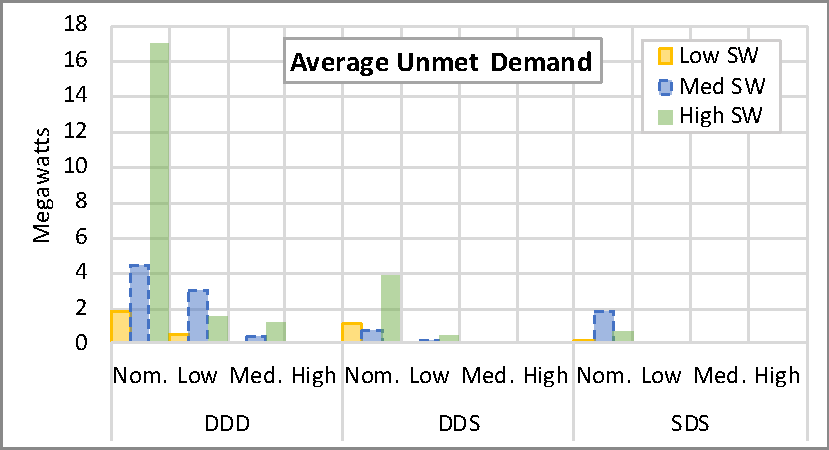
\includegraphics[trim={5mm 2mm 3mm 2mm}, clip, scale=.6]{./figures/avg_unmet_demand.pdf}
\hspace{5mm}
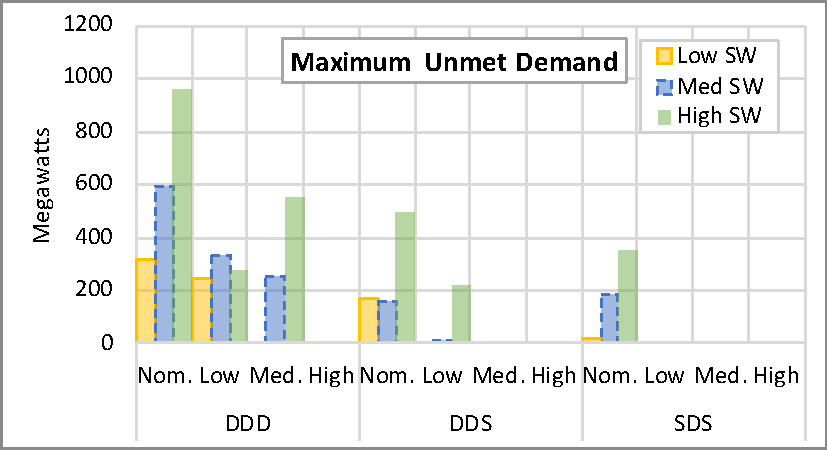
\includegraphics[trim={5mm 2mm 3mm 2mm}, clip, scale=.6]{./figures/max_unmet_demand.pdf}
\caption{Average and maximum unmet demand amounts under different reserve requirements and operations planning strategies.}
\label{sec:experiments:fig:unmet_demand}
\end{figure}

\paragraph{Reliance on ST-UC} 

\paragraph{Over Generation and Renewable Curtailment}

\subsection{Economic Impact} Figure \ref{sec:experiments:fig:avg_daily_cost} demonstrates the average daily operating-costs recorded in our experiments\footnote{This figure neglects the cost of fulfilling the unmet demands reported in the earlier sections.}. In line with our expectations, increased renewable integration leads to lower costs whereas increased reserve requirements have the opposite effect. 
\begin{figure}[h!]
\centering
% trim={<left> <lower> <right> <upper>}
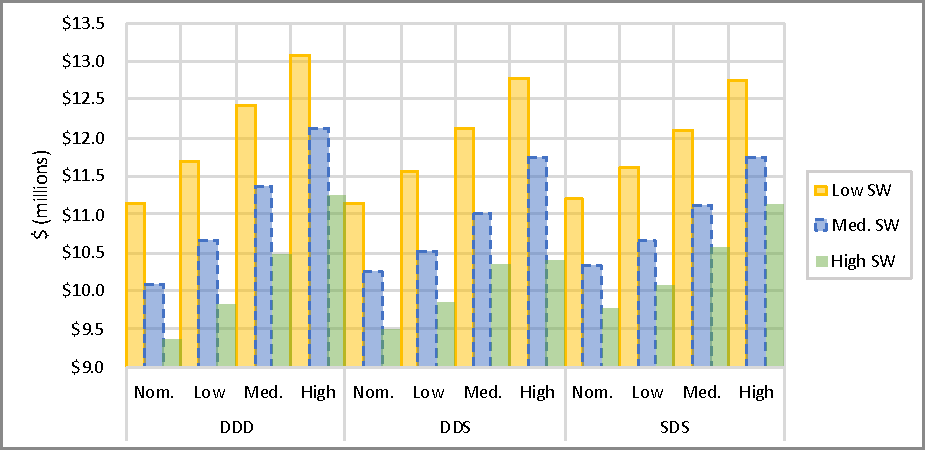
\includegraphics[trim={5mm 2mm 2mm 2mm}, clip, scale=1]{./figures/avg_daily_cost.pdf}
\caption{Average daily operating cost of the power system under different reserve requirements and operations planning strategies.}
\label{sec:experiments:fig:avg_daily_cost}
\end{figure} 

Next, we focus on cases examples where the network demand is seamlessly fulfilled. In particular, in Figure \ref{sec:experiments:fig:avg_daily_cost_demand_met}, we demonstrate the operating costs for the minimum reserve-requirement levels, subject to zero unmet demand. 
\begin{figure}[h!]
\centering
% trim={<left> <lower> <right> <upper>}
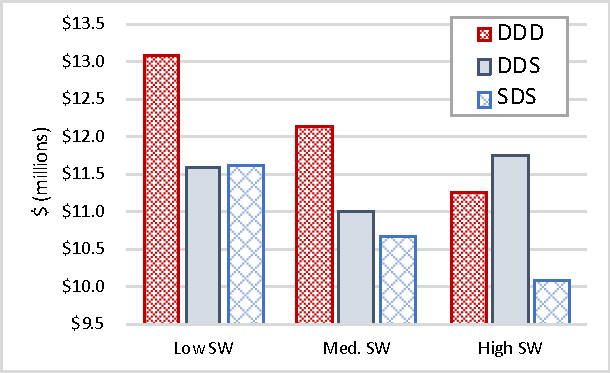
\includegraphics[trim={5mm 2mm 2mm 2mm}, clip, scale=1]{./figures/cost_vs_RI.pdf}
\caption{Average daily operating cost of the power system under all operations planning strategies (only the minimum reserve requirements leading to zero unmet demand are considered).}
\label{sec:experiments:fig:avg_daily_cost_demand_met}
\end{figure} 

\begin{figure}[h!]
\centering
% trim={<left> <lower> <right> <upper>}
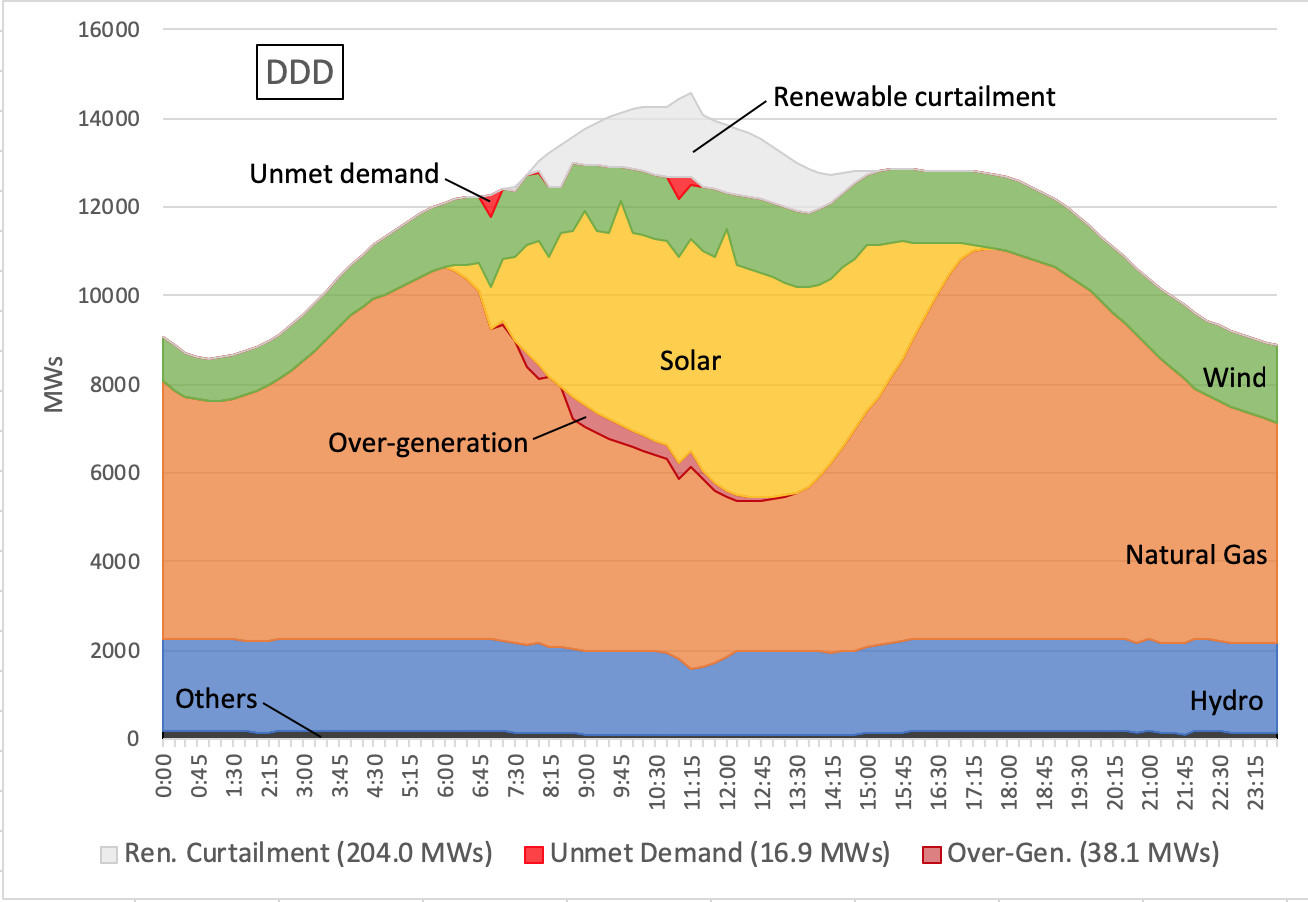
\includegraphics[trim={5mm 2mm 3mm 3mm}, clip, height=6cm]{./figures/ddd_gen_mix.png}
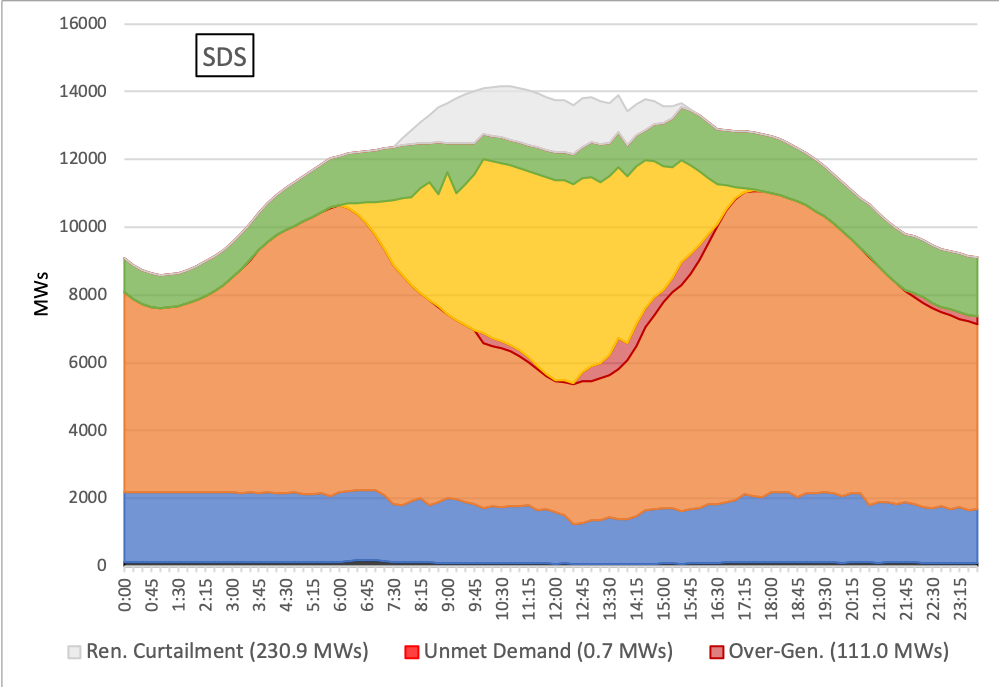
\includegraphics[trim={5mm 2mm 3mm 2mm}, clip, height=6cm]{./figures/sds_gen_mix.png}
\caption{Caption pending}
\label{sec:experiments:fig:generation_mix}
\end{figure} 


\subsection{Environmental Impact}

%It seems like stochastic models do a sufficiently good job in reducing the unmet demand in the planning process. While meeting the whole demand, stochastic models do not significantly sacrifice from costs, and may indeed perform better in certain cases. However, the cautiousness of stochastic models leads to both over-generation and renewable curtailment under high-renewable settings. This reveals a tradeoff: “greedily consuming a lot of renewable supply and not over-generating, versus risking parts of the system to shed load”.
%
%I’ve also prepared some pivot tables under high-renewable scenario. It seems like SDS (and also DDS) reduces the time-averaged commitment of natural gas generators, uses somewhat less Hydro but more Natural Gas production. This seemed a bit confusing to me: Why would you reduce the # of committed natural gas generators, but let the committed ones produce more? Because this clearly reduces your system-wide ramping capabilities? The answer, turns out, lies on the fact that most of these natural gas generators are committed in ST-UC problems. In fact, on average during a day, 15 such generators appear to be committed under DDD. The DDS and SDS reduce this statistic to 9, and 3, respectively. To put it another way, SDS clearly reduces the system's dependence on the ST-UC problems, and the reserve generators that come with it. 
%
%I feel like we have plenty of results to form a decent paper. Can we talk, sometime, what message we are trying to give the readers, and start forming a draft? Along the lines of the thesis, I’d suggest: (1) Explaining the challenges faced by the industry (unmet demand, over-generation, renewable curtailment, costs, pollutants), (2) Describe the framework for analysis, (3) Discuss our findings, (4-Appendix) Optimization methodology. In (3), we should mention that stochastic models reduce unmet demand, produce more over-generation and renewable curtailment, and give a clearer picture on achievable cost- and pollutant-prospects (because stochastic models are more reliable, less greedy).

\pagebreak
\subsubsection*{Counts of words} 
\wordcount

\end{document}
